\documentclass[a4paper,12pt]{article}

\usepackage[english, russian]{babel}

\usepackage[letterpaper,top=2cm,bottom=2cm,left=3cm,right=3cm,marginparwidth=1.75cm]{geometry}
\usepackage{amsmath}
\usepackage{graphicx}
\graphicspath{{pictures/}}
\DeclareGraphicsExtensions{.jpg}
\usepackage[colorlinks=true, allcolors=blue]{hyperref}

\title{Домашняя работа №1}
\author{A-05-19 Карпов Денис}
\date{}

\begin{document}
\maketitle

\section*{\Huge Задание №1}

\subsection*{Построить ДКА, распознающий описанный язык.}

\Large $1.\;L = {\{\omega \in \{a,b,c\}^*|\;|\omega|_c = 1\}}$\newline
Построим регулязное выражение, которое задаёт этот автомат:\newline
\Large$$a^*b^*ca^*b^*$$\newline
Построим на его основе ДКА:\newline
\begin{figure}[h]
\centering
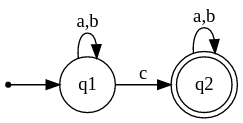
\includegraphics[scale=0.75]{1_1}
\end{figure}

\Large $2.\;L = {\{\omega \in \{a,b\}^*|\;|\omega|_a \le 2,\;|\omega|_b \ge 2\}}$\newline
Разделим описанный язык на $L_1$ и $L_2$, после чего, с помощью прямого произведения ДКА, построим конечный автомат.\newline
\Large $L_1 = {\{\omega \in \{a,b\}^*|\;|\omega|_a \le 2\}}$\newline
\Large $L_2 = {\{\omega \in \{a,b\}^*|\;|\omega|_b \ge 2\}}$\newline
Построим на их основе ДКА:\newline
\begin{figure}[h]
\centering
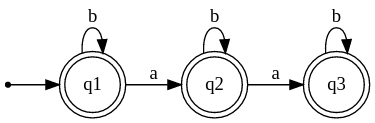
\includegraphics[scale=0.75]{1_2_1}
\caption{$L_1$}
\end{figure}

\begin{figure}[h]
\centering
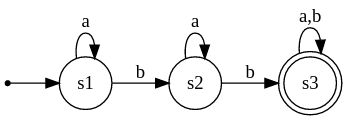
\includegraphics[scale=0.75]{1_2_2}
\caption{$L_2$}
\end{figure}

\begingroup
\raggedleft 
$A_1 = {\langle\sum_1 , Q_1, s_1, T_1, \delta_1 \rangle}$;
$A_2 = {\langle\sum_2 , Q_2, s_2, T_2, \delta_2 \rangle}$\newline
\endgroup
\begingroup
\raggedright 
$A = {\langle\sum , Q, s, T, \delta \rangle}$:
\begin{itemize}
\item $\sum = \sum_1 \cup \sum_2$
\item $Q = Q_1 \times Q_2$
\item $s = \langle s_1 , s_2\rangle$
\item $T = T_1 \times T_2$
\item $\delta(\langle q_1 , q_2\rangle, c) =  \langle \delta_1 (q_1 , c), \delta_2 (q_2, c) \rangle$
\end{itemize}
$\sum = \{q_1, q_2, q_3, s_1, s_2, s_3\}$\newline
\normalsize $Q = \{\langle q_1 , s_1 \rangle ,\langle q_1 , s_2 \rangle ,\langle q_1 , s_3 \rangle , \langle q_2 , s_1 \rangle , \langle q_2 , s_2 \rangle , \langle q_2 , s_3 \rangle , \langle q_3 , s_1 \rangle , \langle q_3 , s_2 \rangle , \langle q_3 , s_3 \rangle \}$\newline
\Large $s = \langle q_1 , s_1 \rangle$\newline
$T = \{\langle q_1 , s_3 \rangle ,\langle q_2 , s_3 \rangle ,\langle q_3 , s_3 \rangle\}$\newline
\begin{center}
\begin{tabular}{ |c|c|c| } 
\hline
  & a & b \\ [0.5ex] 
 \hline
 $\langle q_1 , s_1 \rangle$ & $\langle q_2 , s_1 \rangle$ & $\langle q_1 , s_2 \rangle$ \\ 
 $\langle q_1 , s_2 \rangle $ & $\langle q_2 , s_2 \rangle$ & $\langle q_1 , s_3 \rangle$ \\ 
 $\langle q_1 , s_3 \rangle $ & $\langle q_2 , s_3 \rangle$ & $\langle q_1 , s_3 \rangle$ \\ 
 $\langle q_2 , s_1 \rangle $ & $\langle q_3 , s_1 \rangle$ & $\langle q_2 , s_2 \rangle$ \\ 
 $\langle q_2 , s_2 \rangle $ & $\langle q_3 , s_2 \rangle$ & $\langle q_2 , s_3 \rangle$ \\
 $\langle q_2 , s_3 \rangle $ & $\langle q_3 , s_3 \rangle$ & $\langle q_2 , s_3 \rangle$ \\
 $\langle q_3 , s_1 \rangle $ &  & $\langle q_3 , s_2 \rangle$ \\
 $\langle q_3 , s_2 \rangle $ &  & $\langle q_3 , s_3 \rangle$ \\
 $\langle q_3 , s_3 \rangle $ &  & $\langle q_3 , s_3 \rangle$ \\
 \hline
\end{tabular}
\end{center}
\endgroup
Итоговый ДКА:\newline
\begin{figure}[h]
\centering
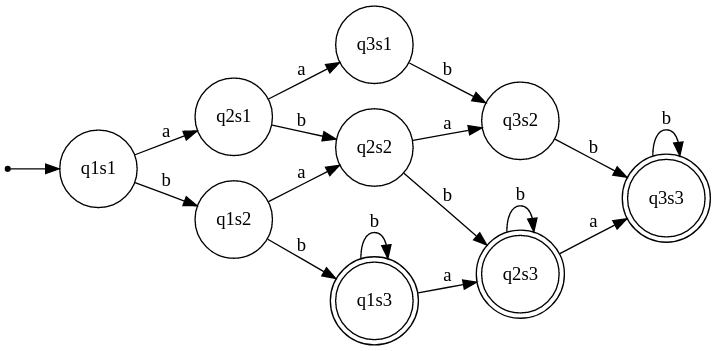
\includegraphics[scale=0.6]{1_2_3}
\end{figure}\newline
$3.\;L = {\{\omega \in \{a,b\}^*|\;|\omega|_a \ne |\omega|_b\}}$\newline
$4.\;L = {\{\omega \in \{a,b\}^*|\;\omega\omega = \omega\omega\omega \}}$\newline
Данный язык представляется исключительно пустым словом: \newline
\begin{figure}[h]
\centering
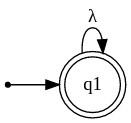
\includegraphics[scale=0.75]{1_4}
\end{figure}\newline

\section*{\Huge Задание №2}
\subsection*{Построить ДКА, распознающий описанный язык, построенный при помощи прямого произведения ДКА и его свойств.}
\Large $2.\;L = {\{\omega \in \{a,b\}^*|\;|\omega|_a \ge 2,\;|\omega|_b \ge 2\}}$\newline
Разделим описанный язык на $L_1$ и $L_2$, после чего, с помощью прямого произведения ДКА, построим конечный автомат.\newline
\Large $L_1 = {\{\omega \in \{a,b\}^*|\;|\omega|_a \ge 2\}}$\newline
\Large $L_2 = {\{\omega \in \{a,b\}^*|\;|\omega|_b \ge 2\}}$\newline
Построим на их основе ДКА:\newline
\begin{figure}[h]
\centering
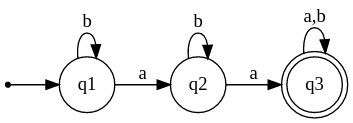
\includegraphics[scale=0.75]{2_1_1}
\caption{$L_1$}
\end{figure}
\begin{figure}[h]
\centering
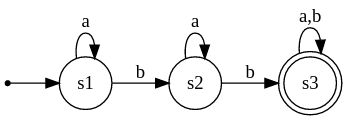
\includegraphics[scale=0.75]{2_1_2}
\caption{$L_2$}
\end{figure}\newline
\begingroup
\raggedleft 
$A_1 = {\langle\sum_1 , Q_1, s_1, T_1, \delta_1 \rangle}$;
$A_2 = {\langle\sum_2 , Q_2, s_2, T_2, \delta_2 \rangle}$\newline
\endgroup
\begingroup
\raggedright 
$A = {\langle\sum , Q, s, T, \delta \rangle}$:
\begin{itemize}
\item $\sum = \sum_1 \cup \sum_2$
\item $Q = Q_1 \times Q_2$
\item $s = \langle s_1 , s_2\rangle$
\item $T = T_1 \times T_2$
\item $\delta(\langle q_1 , q_2\rangle, c) =  \langle \delta_1 (q_1 , c), \delta_2 (q_2, c) \rangle$
\end{itemize}
$\sum = \{q_1, q_2, q_3, s_1, s_2, s_3\}$\newline
\normalsize $Q = \{\langle q_1 , s_1 \rangle ,\langle q_1 , s_2 \rangle ,\langle q_1 , s_3 \rangle , \langle q_2 , s_1 \rangle , \langle q_2 , s_2 \rangle , \langle q_2 , s_3 \rangle , \langle q_3 , s_1 \rangle , \langle q_3 , s_2 \rangle , \langle q_3 , s_3 \rangle \}$\newline
\Large $s = \langle q_1 , s_1 \rangle$\newline
$T = \langle q_3 , s_3 \rangle$\newline
\begin{center}
\begin{tabular}{ |c|c|c| } 
\hline
  & a & b \\ [0.5ex] 
 \hline
 $\langle q_1 , s_1 \rangle$ & $\langle q_2 , s_1 \rangle$ & $\langle q_1 , s_2 \rangle$ \\ 
 $\langle q_1 , s_2 \rangle $ & $\langle q_2 , s_2 \rangle$ & $\langle q_1 , s_3 \rangle$ \\ 
 $\langle q_1 , s_3 \rangle $ & $\langle q_2 , s_3 \rangle$ & $\langle q_1 , s_3 \rangle$ \\ 
 $\langle q_2 , s_1 \rangle $ & $\langle q_3 , s_1 \rangle$ & $\langle q_2 , s_2 \rangle$ \\ 
 $\langle q_2 , s_2 \rangle $ & $\langle q_3 , s_2 \rangle$ & $\langle q_2 , s_3 \rangle$ \\
 $\langle q_2 , s_3 \rangle $ & $\langle q_3 , s_3 \rangle$ & $\langle q_2 , s_3 \rangle$ \\
 $\langle q_3 , s_1 \rangle $ & $\langle q_3 , s_1 \rangle$ & $\langle q_3 , s_2 \rangle$ \\
 $\langle q_3 , s_2 \rangle $ & $\langle q_3 , s_2 \rangle$ & $\langle q_3 , s_3 \rangle$ \\
 $\langle q_3 , s_3 \rangle $ & $\langle q_3 , s_3 \rangle$ & $\langle q_3 , s_3 \rangle$ \\
 \hline
\end{tabular}
\end{center}
\endgroup
Итоговый ДКА: \newline
\begin{figure}[h]
\centering
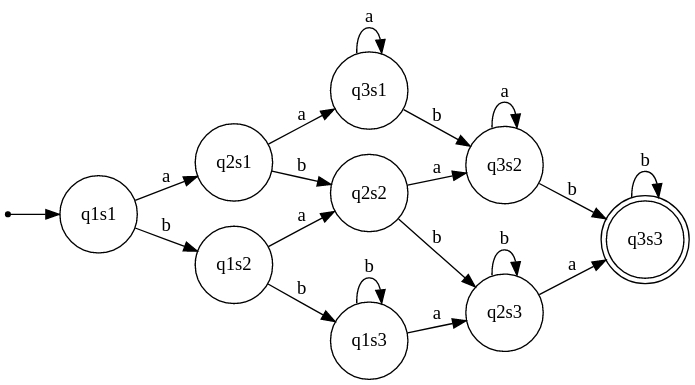
\includegraphics[scale=0.6]{2_1}
\end{figure}
\end{document}